\documentclass[11pt]{article}

% Packages for math and proof writing
\usepackage{amsmath, amssymb, amsthm}
\usepackage{bbm}

% Theorem and proof environments
\newtheorem{theorem}{Theorem}
\newtheorem{lemma}[theorem]{Lemma}
\newtheorem{proposition}[theorem]{Proposition}
\newtheorem{corollary}[theorem]{Corollary}

% Definitions, remarks, etc.
\theoremstyle{definition}
\newtheorem{definition}[theorem]{Definition}
\newtheorem{example}[theorem]{Example}

\theoremstyle{remark}
\newtheorem{remark}[theorem]{Remark}

% Page formatting
\usepackage[margin=1in]{geometry}

%tikz formatting

\usepackage{tikz}
\usepackage{pgfplots}
\pgfplotsset{compat=1.18}
\usepackage{url}

\title{Week 10:\ Null-Hypothesis Significance Testing}
\author{David Kinney}
\date{October 30th, 2025}

\begin{document}

\maketitle

\section{Introduction}
In many areas of philosophy, it is becoming increasingly commonplace to engage directly with contemporary results in empirical science. By this I mean not just knowing the state of the art in the empirical sciences (as many philosophers have for millennia) but also actively keeping up with the literature (i.e., reading papers published in the leading journals) in at least some area of empirical science. In many empirical sciences, null hypothesis significance testing (or, ``NHST'') is the primary means by which justified belief in some conclusion, theory, or hypothesis is established. This is especially true in psychology, which is the primary empirical science with which many philosophers of mind and cognitive science engage.\par

Graduate students in psychology typically receive a \textit{practical} training in NHST. That is, they learn which types of significance tests are used to establish a significant result in specific types of experiments, how to run those significance tests on real data sets in statistical software packages (usually R), and how to interpret the output of these tests. These are all important skills for psychologists and experimental philosophers to have. There are \textit{many} ways to acquire these skills these days, and we won't spend time on doing so this week. Instead, we will focus on the \textit{foundations} of NHST, using probability theory to do so. We will proceed this way for two reasons:\ 1) in my experience, the logic of NHST is sometimes easier for philosophers to digest when it is presented in a foundational way that is grounded in probability theory and ultimately set theory, and 2) for epistemologists, it is important to understand the logic behind one of the primary ways in which justified belief is established in the sciences.\par 


In what follows, I will first present the foundations of NHST for a specific, simple case:\ the two-sample t-test. I will show how this test can be entirely described using probability theory. After this, I will generalize from the case of a two-sample t-test to give a probabilistic description of a larger set of null-hypothesis significance tests. While the material on the Riemann integral and the Gamma function is mathematically dense, you will not need much of it for the problem set.


\section{The Two-Sample t-Test}
\subsection{The Experimental Setup}
Consider a very simple design for an experiment:\ participants are placed into one of two groups, and members of each group are asked to evaluate a stimulus object using a real number. For example, members of one group could be shown a red pair of shoes while members of the other group are shown a blue pair of shoes, with each individual asked to use real numbers to quantify how likely they would be to buy the shoes for \$85. The \textbf{null hypothesis} $H_{0}$ is that there should be no difference between the two groups with respect to the mean of their evaluations.\par

\subsection{A Set-Theoretic Representation}
To represent this set-theoretically, let $n_{1}\in\mathbbm{N}$ be the number of people in the first group and let $n_{2}\in\mathbbm{N}$ be the number of people in the second group. Let $[1,n_{1}]\subset\mathbbm{N}$ be the set of all natural numbers greater than or equal to $1$ and less than or equal to $n_{1}$. Let $[1,n_{2}]\subset\mathbbm{N}$ be the set of all natural numbers greater than or equal to $1$ and less than or equal to $n_{2}$. Let $G_{1}$ be the set of all functions $g_{1}:[1,n_{1}]\rightarrow\mathbbm{R}$. For every $i\in[1,n_{1}]$, $g_{1}(i)$ represents the score assigned to the shoes by the $i$-th member of the first group. For example, if $g_{1}(1)=6$, this means that the first member of the first group assigned the shoes a score of 6; if $g_{1}(2)=4$, this means that the first member of the first group assigned the shoes a score of 4; and so on. Let $G_{2}$ be the set of all functions $g_{2}:[1,n_{2}]\rightarrow\mathbbm{R}$.  For every $i\in[1,n_{2}]$, $g_{2}(i)$ represents the score assigned to the shoes by the $i$-th member of the second group group. For example, if $g_{2}(1)=5$, this means that the first member of the second group assigned the shoes a score of 6; if $g_{2}(2)=7$, this means that the first member of the first group assigned the shoes a score of 7; and so on. Thus, any data set obtained after running this experiment can be represented as a pair $(g_{1},g_{2})\in (G_{1}\times G_{2})$.\par

\subsection{Means and Standard Deviations}
As a next step, we will define functions that calculate the mean score in each of the two groups. Let $\mu_{1}:G_{1}\rightarrow\mathbbm{R}_{\geq1}$ (where $\mathbbm{R}_{\geq1}$ is the set of real numbers greater than or equal to 1) be a function whose value is obtained via the following equation:
$$\mu_{1}(g_{1})=\frac{1}{n_{1}}\sum_{i=1}^{n_{1}}g_{1}(i).$$
This should be read as ``$\frac{1}{n_{1}}$ times the sum of all $f(i)$ for natural numbers $i$ between $1$ and $n_{1}$, inclusive.'' In a nutshell, this is just the average score assigned to the shoes by each member of the first group. Similarly, we define a function $\mu_{2}:G_{2}\rightarrow\mathbbm{R}_{\geq1}$ that is calculated as follows:
$$\mu_{2}(g_{2})=\frac{1}{n_{2}}\sum_{i=1}^{n_{2}}g_{2}(i).$$
Next, we define a \textbf{standard deviation} function $s_{1}:G_{1}\rightarrow\mathbbm{R}_{\geq 0}$ whose value is calculated as follows:
$$s_{1}(g_{1})=\sqrt{\frac{1}{n_{1}-1}\sum_{i=1}^{n_{1}}\left(g_{1}(i)-\mu(g_{1})\right)^{2}}.$$
This provides an absolute measurement of the average extent to which each score assigned to the shoes by a member of the first group deviates from the mean of that group. We use $\frac{1}{n_{1}-1}$ instead of $\frac{1}{n_{1}}$ because once we know the mean $\mu_{1}(g_{1})$ and all but one data point, the final data point can be derived analytically. Thus, $n_{1}-1$ is the number of data points that can freely vary for a given mean, this is also known as the number of \textbf{degrees of freedom} in the calculation of the variance. Similarly, the standard deviation function $s_{2}:G_{2}\rightarrow\mathbbm{R}_{\geq 0}$ can be calculated as follows:
$$s_{2}(g_{2})=\sqrt{\frac{1}{n_{2}-1}\sum_{i=1}^{n_{2}}\left(g_{2}(i)-\mu(g_{2})\right)^{2}}.$$
Thus, we can straightforwardly calculate the mean and standard deviation of the ratings assigned to the shoes by members of each group. Finally, the \textbf{pooled standard deviation function} $s_{p}:(G_{1}\times G_{2})\rightarrow\mathbbm{R}_{\geq0}$ can be calculated as follows:
$$s_{p}((g_{1},g_{2}))=\frac{(n_{1}-1)s_{1}(g_{1})^{2} + (n_{2}-1)s_{2}(g_{2})^{2}}{n_{1}+n_{2} -2}$$
This gives us the overall measure of the variance from the mean across both groups. 

\subsection{The t-Statistic}\label{subsec:tstat}
Equipped with these functions, we can now define a function $t:\Omega\rightarrow\mathbbm{R}$ that is calculated as follows (recall that each element of $\Omega$ is a pair $(g_{1},g_{2})$): 
$$t((g_{1},g_{2}))=\frac{\mu_{1}(g_{1})-\mu_{2}(g_{2})}{s_{p}((g_{1},g_{2}))\sqrt{\frac{1}{n_{1}}+\frac{1}{n_{2}}}}.$$
The value of this equation is known as the \textbf{t-statistic} for a given data set $(g_{1},g_{2})$ obtained from a two-sample t-test. Its value is $0$ when the mean of each group's evaluations of the shoes are identical, with $t$ becoming more positive or negative as the means differ. The denominator term ensures that $t$ gets larger as the variance is small. Thus, if the two groups disagree, but do not vary internally with respect to their evaluations of the shoes, then $t$ will be large.\par 


Consider the product $G_{1}\times G_{2}$, representing the set of all possible experimental outcomes. Consider the set of real numbers $\mathbbm{R}$ and the Borel $\sigma$-algebra $\mathcal{B}$ on $\mathbbm{R}$. Let $\Sigma$ be a set defined so that $S\in\Sigma$ if and only if there exists a $B\in\mathcal{B}$ such that $S=\left\{(g_{1},g_{2})\in(G_{1}\times G_{2}):t((g_{1},g_{2}))\in B\right\}$. Thus, $\Sigma$ contains all and only the sets of data sets whose t-statistics are in some element of the Borel $\sigma$-algebra on the real numbers. It turns out that $\Sigma$ is a $\sigma$-algebra on $G_{1}\times G_{2}$; it is a set of subsets of $G_{1}\times G_{2}$ that contains both $G_{1}\times G_{2}$ and $\emptyset$, and is closed under countable union and intersection. Additionally, the random variable $t$ is measurable with respect to $(G_{1}\times G_{2},\Sigma)$. You will prove both of these facts in the problem set.


\subsection{The t-Distribution}
The next step will be to define a probability distribution $p:\Sigma\rightarrow[0,1]$ such $p(t^{-1}(x))$ is defined for any $x\in\mathbbm{R}$. However, before we can do this, we will have to introduce a few additional mathematical concepts, namely the Riemann integral and the Gamma function.\par 

\subsubsection{The Riemann Integral}
Last week, we discussed the Lebesgue integral. Here, we define a different version of the integral, known as the Riemann integral, named after Bernhard Riemann who we also mentioned last week. Let $h$ be any function whose codomain is the set $\mathbbm{R}$ of all real numbers. Let $a\in\mathbbm{R}$ and $b\in\mathbbm{R}$ be any two real numbers such that $a\leq b$. Let $P$ be a sequence of points $(p_{0},\dots,p_{n})$ such that $p_{1}=a$, $p_{n}=b$, and $p_{i-1}<p_{i}$ for all natural numbers $i$ between $1$ and $n$, inclusive. The sequence $P$ is called a \textbf{partition} of the set of all real numbers in the interval $[a,b]$. The \textbf{norm} $||P||$ of a partition $P$ is given by equation:
$$||P||=\max_{1\leq i\leq n}(p_{i}-p_{i+1}).$$
The right-hand side of this equation should be read as ``the maximum value of $(p_{i}-p_{i+1})$ for any $i$ between 1 and $n$, inclusive.''\par 


\begin{figure}[]
\centering
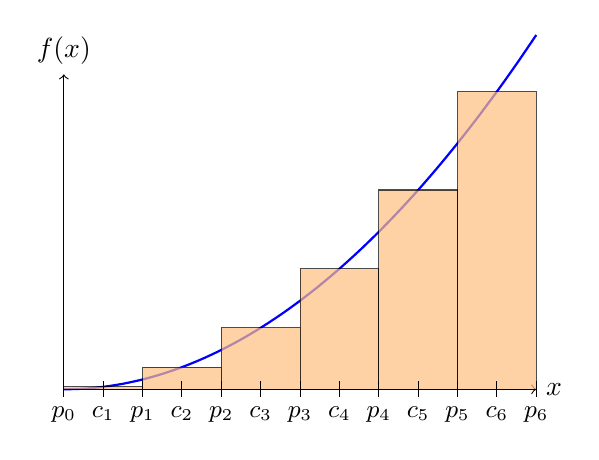
\begin{tikzpicture}[xscale=2, yscale=1]  % LEFT: 6 rectangles
    % Axes
    \draw[->] (0,0) -- (3,0) node[right] {$x$};
    \draw[->] (0,0) -- (0,4) node[above] {$f(x)$};

    % Curve f(x) = 0.5x^2
    \draw[thick, blue, domain=0:3, smooth, variable=\x]
        plot ({\x},{0.5*\x*\x});

    % Rectangles (6 subintervals)
    \foreach \a/\b/\c in {0/0.5/0.25,0.5/1/0.75,1/1.5/1.25,1.5/2/1.75,2/2.5/2.25,2.5/3/2.75}{
        \draw[fill=orange!50, opacity=0.7] (\a,0) rectangle (\b, {0.5*\c*\c});
    }

    % Partition points p0...p6
    \foreach \x/\label in {0/p_0,0.5/p_1,1/p_2,1.5/p_3,2/p_4,2.5/p_5,3/p_6}{
        \draw (\x,0.1) -- (\x,-0.1) node[below] {\small $\label$};
    }

    % Sample points c1...c6
    \foreach \x/\label in {0.25/c_1,0.75/c_2,1.25/c_3,1.75/c_4,2.25/c_5,2.75/c_6}{
        \draw (\x,0.1) -- (\x,-0.1) node[below] {\small $\label$};
    }

\end{tikzpicture}
\hspace{1cm} % space between plots
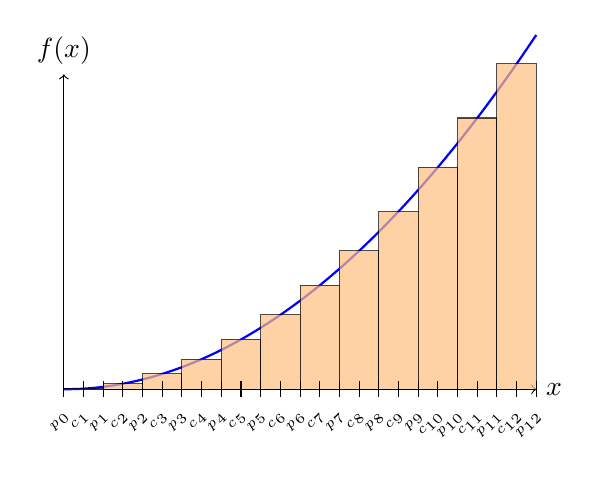
\begin{tikzpicture}[xscale=2, yscale=1]  % RIGHT: 12 rectangles
    % Axes
    \draw[->] (0,0) -- (3,0) node[right] {$x$};
    \draw[->] (0,0) -- (0,4) node[above] {$f(x)$};

    % Curve f(x) = 0.5x^2
    \draw[thick, blue, domain=0:3, smooth, variable=\x]
        plot ({\x},{0.5*\x*\x});

    % Rectangles (12 subintervals)
    \foreach \i in {1,...,12}{
        \pgfmathsetmacro\a{(\i-1)*0.25}
        \pgfmathsetmacro\b{\i*0.25}
        \pgfmathsetmacro\c{(\a+\b)/2}
        \draw[fill=orange!50, opacity=0.7] (\a,0) rectangle (\b,{0.5*\c*\c});
    }

    % Partition points p0...p12 (tilted)
    \foreach \i in {0,...,12}{
        \pgfmathsetmacro\x{0.25*\i}
        \draw (\x,0.1) -- (\x,-0.1);
        \node[below, rotate=45, anchor=north east] at (\x,-0.1) {\tiny $p_{\i}$};
    }

    % Sample points c1...c12 (tilted)
    \foreach \i in {1,...,12}{
        \pgfmathsetmacro\x{0.25*(\i-0.5)}
        \draw (\x,0.1) -- (\x,-0.1);
        \node[below, rotate=45, anchor=north east] at (\x,-0.1) {\tiny $c_{\i}$};
    }

\end{tikzpicture}

\caption{Rectangles under $h(x)=\frac12 x^2$ for the interval $[0,3]$. In the left chart, the height of each rectangle is $h(c_{i})$ for $1\leq i\leq 6$, and the length of each rectangle is given by $(p_i-p_{i-1})$. Thus, the Riemann sum $\sum_{i=1}^{n}h(c_{i})(p_{i}-p_{i-1})$ is equal to the area of these six rectangles. As we add more points to the partition partition $(p_{0},\dots,p_{n})$ of $[0,3]$ (so that $||P||$ is smaller), the area of these rectangles more closely approximates the area under the curve, as demonstrated by the right chart. The Riemann integral, when it exists, is the limit of the area of the rectangles generated by an increasingly fine-grained partition.}\label{fig:riemann}
\label{fig:riemann_comparison}
\end{figure}

For each $p_{i}$ in the partition such that $i\geq1$, let $c_{i}$ be a real number, known as a \textbf{sample point}, such that $p_{i-1}\leq c_{i}\leq p_{i}$. For any function $h$ whose domain contains $[a,b]$ as a subset and whose codomain is the real numbers, partition $P$, and sequence of sample points $C=(c_{1},\dots,c_{n})$, the \textbf{Riemann sum} is given by the equation:
$$S(h,P,C)=\sum_{i=1}^{n}h(c_{i})(p_{i}-p_{i-1}).$$
This allows us to define the notion of Riemann integrability for a function whose domain contains $[a,b]$ as a subset and whose codomain is the real numbers:
\begin{definition}
    A function $h$ whose domain contains $[a,b]$ as a subset and whose codomain is the real numbers is \textbf{Riemann integrable} for the interval $[a,b]\subseteq\mathbbm{R}$, where $a$ and $b$ are real numbers such that $a\leq b$, if and only if there exists a real number $I\in\mathbbm{R}$ and a real number $\delta>0$ such that for all real numbers $\epsilon>0$ and all partitions $P$ of $[a,b]$ such that $||P||<\delta$, and all sample points $C$, $|S(h,P,C)-I|<\epsilon$. It turns out that if such an $I$ exists, it exists uniquely.
\end{definition}
\noindent
This definition allows us to define the proper Riemann integral for a function $h$ whose domain is the real numbers:
\begin{definition}
    For any Riemann integrable function, its \textbf{proper Riemann integral} on the interval $[a,b]$ where $a$ and $b$ are real numbers such that $a\leq b$, is given by the equation:
    $$\int_{a}^{b}h(x)\textrm{d}x = I,$$
    where $I$ is the unique real number such that for all real numbers $\epsilon>0$ and all partitions $P$ of $[a,b]$ such that $||P||<\delta$ for some real number $\delta>0$, and all sample points $C$, $|S(h,P,C)-I|<\epsilon$.
\end{definition}
\noindent
The left-hand side of the equation above should read as ``the integral of $h$ with respect to $x$ from $a$ to $b$.'' Fig.~\ref{fig:riemann} illustrates how this Riemann integral approximates the area under the function $h$, when $h$ takes positive values.


Sometimes, we are interested in the integral of a function $h$ on the set of all real numbers greater than or equal to some $a\in\mathbbm{R}$. This integral, which is one example of an \textit{im}proper Riemann integral, is defined as follows:
\begin{definition}
    Let $a\in\mathbbm{R}$ be any real number. Let $h$ be a function such that, for any real number $b\geq a$, its domain contains $[a,b]$ as a subset, its codomain is the real numbers, and it is Riemann integrable on the interval $[a,b]$. If there exists a unique limit $L$ such that, for any $\epsilon>0$, there exists a $B\in\mathbbm{R}$ such that
    $$\left|\int_{a}^{b}h(x)\textrm{d}x-L\right|<\epsilon$$
    for all $b\geq B$, then the \textbf{improper Riemann integral} of $h$ on the interval $[a,\infty]$ is given by the equation:
    $$\int_{a}^{\infty}h(x)\textrm{d}x=L.$$
\end{definition}
\noindent
Thus, the integral of $h$ on the set of all real numbers grater that $a$ is just the unique real number $L$ such that $\int_{a}^{b}h(x)\textrm{d}x$ can be made arbitrarily close to $L$ be incrasingly $b$. We use a very similar strategy to define the integral of the function $h$ on the set of all real numbers less than or equal to some $a\in\mathbbm{R}$:
\begin{definition}
    Let $a\in\mathbbm{R}$ be any real number. Let $h$ be a function such that, for any real number $b\leq a$, its domain contains $[b,a]$ as a subset, its codomain is the real numbers, and it is Riemann integrable on the interval $[b,a]$. If there exists a unique limit $L$ such that, for any $\epsilon>0$, there exists a $B\in\mathbbm{R}$ such that
    $$\left|\int_{b}^{a}h(x)\textrm{d}x-L\right|<\epsilon$$
    for all $b\leq B$, then the improper Riemann integral of $h$ on the interval $[-\infty,a]$ is given by the equation:
    $$\int_{-\infty}^{a}h(x)\textrm{d}x=L.$$
\end{definition}
\noindent
Finally, we can combine these two definitions to define the improper Riemann integral of a function on all real numbers:
\begin{definition}
    Let $h$ be a function such that its domain and codomain are the real numbers, and, for any $a\in\mathbbm{R}$, the improper Riemann integral on the intervals $[-\infty,a]$ and $[a,\infty]$ exist. The improper Riemann integral on the interval $[-\infty,\infty]$ is given by the equation:
    $$\int_{-\infty}^{\infty}h(x)\textrm{d}x = \int_{-\infty}^{a}h(x)\textrm{d}x + \int_{a}^{\infty}h(x)\textrm{d}x.$$
\end{definition}
\noindent
For reasons that will become clear shortly, it is important in many NHST contexts that we be able to say that a function's improper Riemann integral on the interval $[-\infty,\infty]$ is well-defined and equal to 1.\par 


\subsubsection{The Gamma Function}
The part of the \textbf{Gamma function} defined on the positive reals, which plays a crucial role in two-sample t-tests, is a function $\Gamma:\mathbbm{R}_{>0}\rightarrow\mathbbm{R}_{>0}$ with the following definition:
$$\Gamma(z)=\int_{0}^{\infty}x^{z-1}e^{-x}\textrm{d}x,$$
where $e$ is \textbf{Euler's number}, which is a well-known mathematical constant with a number of important applications. Note that the domain of the \textit{full} definition of the Gamma function is the set of all complex numbers apart from the complex numbers that match the negative integers, but we don't need this full definition to calculate the t-distribution.

\subsubsection{The t-Distribution}
We are nearly in a position to define a probability distribution on the set $\Sigma$ defined above. However, we will first have to define just a few more terms. First, a \textbf{probability density function} for the random variable $V$ is a function $f_{V}:\mathbbm{R}\rightarrow\mathbbm{R}_{\geq0}$ such that if $[a,b]$ is the set of all real numbers between any $a\in\mathbbm{R}$ and $b\in\mathbbm{R}$, $(\Omega,\Sigma)$ is a measurable space, and $V:\Omega\rightarrow\mathbbm{R}$ is a random variable that is measurable with respect to $(\Omega,\Sigma)$, then there is a probability distribution $p:\Sigma\rightarrow[0,1]$ such that
$$p(\{\omega\in\Omega:V(\omega)\in [a,b]\})=\int_{a}^{b}f_{V}(x)\textrm{d}x,$$
where the right-hand side of this equation is a Riemann integral. In other words, the probability that $V$ takes a value in the interval $[a,b]$ is equal to the Riemann integral of the probability density function $f_{V}$ over the same interval.\par 

Let us consider again the random variable $t:(G_{1}\times G_{2})\rightarrow \mathbbm{R}_{\geq0}$, defined in Sec.~\ref{subsec:tstat} above. Let $\nu=n_{1}+n_{2}-2$. We define a probability density function $f_{t}:\mathbbm{R}\rightarrow\mathbbm{R}_{\geq0}$ that is calculated as follows:
$$f_{t}(x)=\frac{\Gamma\left(\frac{\nu+1}{2}\right)}{\sqrt{\pi\nu}\Gamma\left(\frac{\nu}{2}\right)}\left(1+\frac{x^{2}}{\nu}\right)^{\frac{-\nu+1}{2}}.$$
For our purposes, it is not important to know the details of how this probability density function derived. What \textit{is} important is to know that it defines a very natural probability distribution over $\Sigma$, \textit{under the null hypothesis that the two groups should have the same mean}. To see this, let us define a probability distribution $p_{H_{0}}:\Sigma\rightarrow[0,1]$, such that for any set $S\in\Sigma$, $p_{H_{0}}(S)$ is the probability of our experiment producing a result in $S$, under the null hypothesis that there should be no difference in means between the two groups' evaluations of the shoes.\par 


The key property of this probability distribution is that for any set $[a,b]$ containing all the real numbers between $a$ and $b$, inclusive, the following holds:
$$p_{H_{0}}\left(\{(g_{1},g_{2})\in G_{1}\times G_{2}: t((g_{1},g_{2}))\in[a,b]\}\right)=\int_{a}^{b}f_{t}(x)\textrm{d}x.$$
The following facts demonstrate that the triple $(G_{1}\times G_{2},\Sigma,p_{H_{0}})$, is a probability space, since $p_{H_{0}}$ satisfies Kolmogorov's probability axioms:
\begin{enumerate}
    \item For any result $(g_{1},g_{2})\in G_{1}\times G_{2}$ of our experiment, $t((g_{1},g_{2}))$ must take some value. Thus, the set of possible outcomes of the experiment $G_{1}\times G_{2}$ can be re-written as 
    $$\{(g_{1},g_{2})\in G_{1}\times G_{2}: t((g_{1},g_{2}))\in[-\infty,\infty]\}.$$
    Thus, 
    $$p_{H_{0}}(G_{1}\times G_{2})=\int_{-\infty}^{\infty}f_{t}(x)\textrm{d}x.$$
    It turns out that:
    $$p_{H_{0}}(G_{1}\times G_{2})=\int_{-\infty}^{\infty}f_{t}(x)\textrm{d}x=1.$$

    \item For any $x$, $f_{t}(x)$ is positive. Thus, for any real interval $[a,b]$, 
    $$p_{H_{0}}\left(\{(g_{1},g_{2})\in G_{1}\times G_{2}: t((g_{1},g_{2}))\in[a,b]\}\right)=\int_{a}^{b}f_{t}(x)\textrm{d}x\geq 0,$$
    with $p_{H_{0}}\left(\{(g_{1},g_{2})\in G_{1}\times G_{2}: t((g_{1},g_{2}))\in[a,b]\}\right)=0$ if and only if $a=b$. 

    \item Let $\mathcal{S}$ be a countable set of disjoint elements of $\Sigma$ such that for any $S\in\mathcal{S}$, $$S=\{(g_{1},g_{2})\in(G_{1}\times G_{2}):t((g_{1},g_{2}))\in[a_{S},b_{S}]\},$$
    where $[a_{S},b_{S}]$ is the set of all real numbers between $a_{S}$ and $b_{S}$, inclusive. Since no two elements of $\mathcal{S}$ contain the same elements, no two intervals $[a_{S},b_{S}]$ overlap. Thus,
    $$p_{H_{0}}(\cup\mathcal{S})=\sum_{S\in\mathcal{S}}\int_{a_{S}}^{b_{S}}f_{t}(x)\textrm{d}x=\sum_{S\in\mathcal{S}}p_{H_{0}}(\{(g_{1},g_{2})\in(G_{1}\times G_{2}):t((g_{1},g_{2}))\in[a_{S},b_{S}]\}).$$
\end{enumerate}
This shows that $(G_{1}\times G_{2},\Sigma,p_{H_{0}})$ is indeed a probability space. To see why it makes sense as a natural probability space for representing the probability of getting different outcomes from our experiment when each group's mean evaluation of the shoes should be equal, consider the visualization of the $t$-distribution shown in Fig.~\ref{fig:tdist}. Note that the probability of obtaining a t-statistic between any two points on the $x$-axis is given by the area under the curve between those two points. As the two points in question get further from zero, this area gets smaller. Thus, all else being equal, greater probability is assigned to sets of outcomes that include, or are close to, the possibility that there is no difference in means between the two groups.\par 


\pgfmathdeclarefunction{tpdf}{2}{%
  % #1 = x, #2 = nu
  \pgfmathparse{gamma((#2+1)/2) / (sqrt(#2*pi) * gamma(#2/2)) * (1 + (#1)^2 / #2)^(-(#2+1)/2)}%
}

\begin{figure}[]
\centering
\begin{tikzpicture}
  \begin{axis}[
    width=12cm,
    height=7cm,
    axis lines=left,
    xlabel={$t$},
    ylabel={density},
    domain=-5:5,
    samples=301,
    ymin=0,
    ymax=0.45,
    legend pos=north east,
    legend cell align=left,
    every axis plot/.append style={very thick},
    ticklabel style={font=\small},
    label style={font=\small}
  ]

  % t-distribution nu=5
  \addplot[blue] ({x}, {0.3796 * (1 + x^2 / 5)^(-3)}); 

  \end{axis}
\end{tikzpicture}
\caption{The t-distribution with $\nu=5$.}\label{fig:tdist}
\end{figure}


\subsection{Obtaining p-Values}
Suppose we have run our experiment, and obtained the value of the t-statistic for our observed data set. We now seek to calculate the \textbf{p-value} of our results. In a \textbf{two-tailed} t-test, this is the probability, under the assumption that the null hypothesis is true, of obtaining a value for $t$ whose absolute value is greater than or equal to the absolute value of the t-statistic for the data that we actually observed. To formalize this, let $(g^{*}_{1},g^{*}_{2})$ be our observed data set, and let $t^{*}=t((g^{*}_{1},g^{*}_{2}))$ be the value of the $t$-statistic that we actually obtain. We want to calculate the probability, under the null hypothesis, of observing any data set $(g_{1},g_{2})$ such that $|t((g_{1},g_{2}))|\in[|t^{*}|,\infty]$.\par 

Concretely, if $t^{*}$ is positive, then the p-value associated with a test that returns to the t-statistic $t^{*}$ is the probability
$$p_{H_{0}}(\{(g_{1},g_{2})\in(G_{1}\times G_{2}):t((g_{1},g_{2}))\in [t^{*},\infty]\} \ \text{or} \ -t((g_{1},g_{2}))\in [-\infty,-t^{*}]\}).$$
This can be re-written as:
$$p_{H_{0}}(\{(g_{1},g_{2})\in(G_{1}\times G_{2}):t((g_{1},g_{2}))\in [t^{*},\infty]\} \cup \{(g_{1},g_{2})\in(G_{1}\times G_{2}):-t((g_{1},g_{2}))\in [-\infty,-t^{*}]\}).$$
Countable additivity means we can re-write this as
\begin{multline*}
    p_{H_{0}}(\{(g_{1},g_{2})\in(G_{1}\times G_{2}):t((g_{1},g_{2}))\in [t^{*},\infty]\}) \\ + p_{H_{0}}(\{(g_{1},g_{2})\in(G_{1}\times G_{2}):-t((g_{1},g_{2}))\in [-\infty,-t^{*}\}).
\end{multline*}
Finally, the definition of $p_{H_{0}}$ allows us to calculate this as the sum of the Riemann integrals
$$\int_{t}^{\infty}f_{t}(x)\textrm{d}x + \int_{-\infty}^{-t}f_{t}(x)\textrm{d}x,$$
where $f_{t}$ is the probability density function for the t-distribution. This, is the p-value for our two-sample, two-tailed t-test. On the other hand, if $t^{*}$ is negative, then $t^{*}$ is the probability
$$p_{H_{0}}(\{(g_{1},g_{2})\in(G_{1}\times G_{2}):t((g_{1},g_{2}))\in [-t^{*},\infty]\} \ \text{or} \ -t((g_{1},g_{2}))\in [-\infty,t^{*}]\}).$$
This can be re-written as:\par
$$p_{H_{0}}(\{(g_{1},g_{2})\in(G_{1}\times G_{2}):t((g_{1},g_{2}))\in [-t^{*},\infty]\} \cup \{(g_{1},g_{2})\in(G_{1}\times G_{2}):-t((g_{1},g_{2}))\in [-\infty,t^{*}]\}).$$
\begin{multline*}
    p_{H_{0}}(\{(g_{1},g_{2})\in(G_{1}\times G_{2}):t((g_{1},g_{2}))\in [-t^{*},\infty]\}) \\ + p_{H_{0}}(\{(g_{1},g_{2})\in(G_{1}\times G_{2}):-t((g_{1},g_{2}))\in [-\infty,t^{*}\}).
\end{multline*}
Finally, the definition of $p_{H_{0}}$ allows us to calculate this as the sum of the Riemann integrals
$$\int_{-t}^{\infty}f_{t}(x)\textrm{d}x + \int_{-\infty}^{t}f_{t}(x)\textrm{d}x.$$
Thus, we can calculate the p-value for any result $(g_{1},g_{2})$ of our simple experiment.\par 

Low p-values are associated with experimental results such that those results, or results that yield a more extreme p-value, are less likely to occur if the null hypothesis is true. Thus, obtaining a low p-value is typically taken to be evidence that the null hypothesis is false. Recall that in a two-sample t-test, the null hypothesis is that means of the measurements between two groups (in this case, the mean evaluation of the two pairs of shoes) should be identical. So, a low p-value supports the conclusion that there should be a difference in means between the two groups (i.e., because one color of shoe is more desirable). Typically, empirical scientists set a threshold such that, if they obtain a p-value below that threshold, they will say that they have a \textbf{significant result} and reject the null hypothesis. Otherwise, they will say that they do not have a significant result, and therefore fail to reject the null hypothesis.\par 

\section{NHST Generalized}
Generalizing from this case, we can construct a more general algorithm for running a null hypothesis significance test on the results of an experiment and calculating a p-value:
\begin{enumerate}
    \item Define a space $\Omega$ of possible outcomes of the experiment.

    \item Define a \textbf{test statistic}, which is a random variable $V:\Omega\rightarrow\mathbbm{R}$.

    \item Let $\mathcal{B}$ be the Borel $\sigma$-algebra on $\mathbbm{R}$, and let $\Sigma$ be a set such that $S\in\Sigma$ if and only if there exists a $B\in \mathcal{B}$ such that $S=\{\omega\in\Omega:V(\omega)\in B\}$. This $\Sigma$ will be a $\sigma$-algebra on $\Sigma$, and the random variable $V$ will be measurable with respect to $(\Omega,\Sigma)$.

    \item Define a probability density function $f_{V}:\mathbbm{R}\rightarrow\mathbbm{R}$ such that, for any set $[a,b]$ consisting of all real numbers greater than $a$ or less than $b$, inclusive, $$p_{H_{0}}(\{\omega\in\Omega:V(\omega)\in[a,b]\})=\int_{a}^{b}f_{V}(x)\textrm{d}x,$$
    where $p_{H_{0}}:\Sigma\rightarrow[0,1],$ is in some sense, a ``natural'' distribution over sets of possible outcomes of our experiment, under the assumption that \textit{some} null hypothesis $H_{0}$ is true.
\end{enumerate}
While this doesn't cover every conceivable null hypothesis significance test (e.g., some test statistics may take natural or integer values rather than real values), this description does cover a large class of them. Note that what counts as a good choice of null hypothesis $H_{0}$ for a particular experiment, and what counts as a natural choice of probability distribution $p_{H_{0}}$ for representing probabilities of sets of outcomes under the null distribution $H_{0}$, is, in some sense, in the eye of the beholder. Having said this, one often sees theorems proved establishing that a particular probability distribution $p_{H_{0}}$ satisfies certain key properties that we might intuitively think that a null hypothesis distribution should have.\par 

\section{Conclusion}
As mentioned in the introduction, simple null hypothesis significance tests are now very easy to run using different software packages. Thus, for many working scientists, it is not practically necessary to understand them with as much detail as we have gone into in this reading. However, for philosophy of science and epistemology, it is very useful to understand the logic and assumptions that go into running null hypothesis significance tests, especially as they are primary means by which scientists establish justified beliefs in the significance of experimental results.\par 

\section*{Problem Set}

\begin{enumerate}
\item Prove that in a two-sample, two-tailed t-test, if the observed data $(g^{*}_{1},g^{*}_{2})$ is such that $\mu_{1}(g_{1})=\mu_{2}(g_{2})$, then the p-value for the t-test is 1.



\item Consider the product $G_{1}\times G_{2}$, representing the set of all possible experimental outcomes of a two-sample t-test with group sizez $n_{1}$ and $n_{2}$. Consider the set of real numbers $\mathbbm{R}$ and the Borel $\sigma$-algebra $\mathcal{B}$ on $\mathbbm{R}$. Let $\Sigma$ be a set defined so that, $S\in\Sigma$ if and only if there exists a $B\in\mathcal{B}$ such that $S=\left\{(g_{1},g_{2})\in(G_{1}\times G_{2}):t((g_{1},g_{2}))\in B\right\}$. Thus, $\Sigma$ contains all and only the sets of data sets whose t-statistics are in some element of the Borel $\sigma$-algebra on the real numbers. Prove that:
\begin{enumerate}
    \item $\Sigma$ is a $\sigma$-algebra. (\textit{Hint: Use the fact that $\mathcal{B}$ is a $\sigma$-algebra.})

    \item The random variable $t:(G_{1}\times G_{2})\rightarrow\mathbbm{R}$ is measurable with respect to $(G_{1}\times G_{2},\Sigma)$.
\end{enumerate}

\end{enumerate}

\end{document}
